\section{Vorgehen der Literaturrecherche}
\label{sec:VorgehenLiteraturrecherche}
Unter einer Literaturrecherche versteht man das strukturierte Zusammentragen, Beschreiben und Erklären von wissenschaftlicher Literatur \cite{cooper_organizing_1988}. Hierbei können Methoden, Modelle oder Theorien im Vordergrund stehen, wogegen es eine Literaturrecherche gleichzeitig auch ermöglicht, den aktuellen Stand der Forschung zusammenzufassen. Somit lässt sich auch aufdecken, an welcher Stelle in einem Forschungsfeld noch Wissenslücken bestehen \cite{cooper_organizing_1988, Webster2002AnalyzingTP}.

\begin{figure}
    \centering
    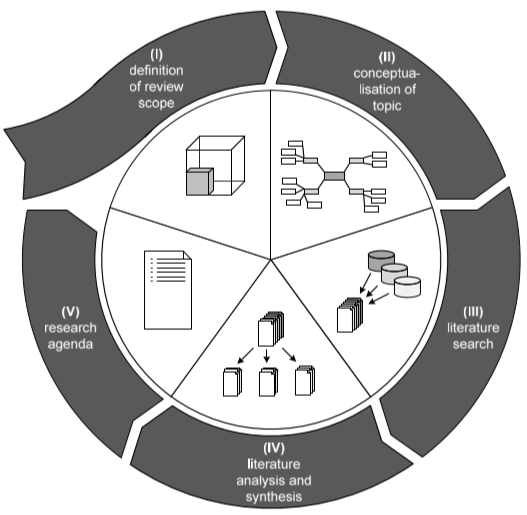
\includegraphics[scale=0.85]{pic/MA-Bilder/Model_vom_Brooke.PNG}
    \caption{Vorgehen einer strukturierten Literaturrecherche, entnommen aus \cite{vom_Brooke_2009}}
    \label{Fig:vomBrocke}
\end{figure}

Für eine Literaturrecherche stehen unterschiedlichste Vorgehensmodelle zur Verfügung. Diese Masterarbeit orientiert sich jedoch grob an dem Vorgehen von \cite{vom_Brooke_2009}, da dieses von mehreren wirtschaftsinformatiknahen Forschern im deutschsprachigen Raum entwickelt wurde. Die grobe Struktur des Vorgehensmodells ist in Abbildung \ref{Fig:vomBrocke} zu sehen. Die Literaturrecherche nach \cite{vom_Brooke_2009} umfasst die \emph{Definition des
Umfangs der Literaturrecherche}, \emph{Konzeptualisierung des Themas}, \emph{Literaturrecherche},
\emph{Literaturanalyse und -synthese} und \emph{Forschungsplanung}. Bei einzelnen Phasen der Literaturrecherche wird weiter noch auf Erkenntnisse von \cite{cooper_organizing_1988}, \cite{Brink.2013} und \cite{Webster2002AnalyzingTP} zurückgegriffen, was in den nachfolgenden Unterkapiteln erläutert wird.